\section{Introducción}
Las celdas de combustible son sistemas electroquímicos que generan electricidad a partir de la energía química de un combustible, mediante procesos de oxidación y reducción. Su principal atractivo como fuente de energía eléctrica radica en su capacidad de ofrecer una conversión más eficiente en comparación con los métodos convencionales basados en ciclos termoeléctricos \cite{cec}. Por su parte, un convertidor DC-DC es un equipo electrónico diseñado para modificar el voltaje de corriente continua, adaptándolo de un nivel a otro. Esta función es especialmente valiosa, ya que en muchos dispositivos electrónicos es común que distintos componentes necesiten distintos niveles de tensión para operar correctamente. Gracias a su versatilidad, estos convertidores pueden elevar, reducir o invertir el voltaje, según lo exijan las condiciones del sistema \cite{juanito}.

En este informe se aborda el diseño, modelación e implementación de un sistema de control para un sistema híbrido conformado por una celda de combustible y un banco de baterías (convertidor DC-DC). El objetivo principal de la implementación de este sistema es regular el voltaje de una carga eléctrica a un valor de referencia de 250 V. La celda de combustible se caracteriza por una respuesta dinámica lenta pero capaz de entregar alta potencia, mientras que el sistema de baterías presenta una dinámica rápida pero con capacidad limitada para operación continua.

\begin{figure}
    \centering
    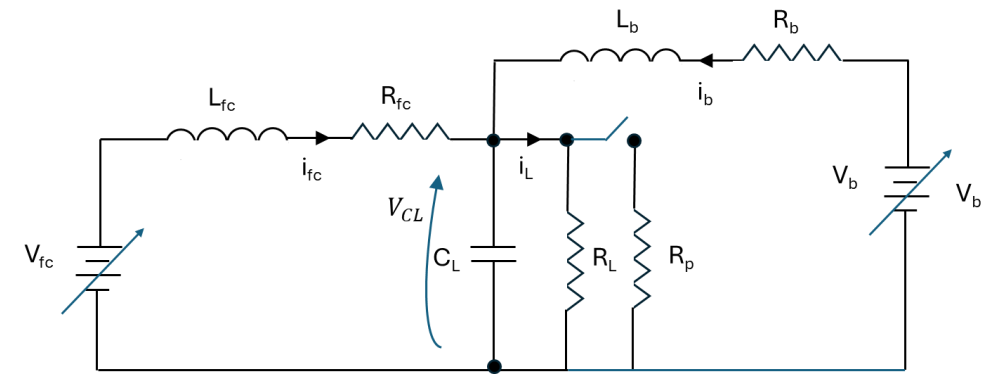
\includegraphics[width=0.7\linewidth]{img/circuito.png}
    \caption{Sistema MIMO, donde se debe controlar V$_{\text{CL}}$ a 250V.}
    \label{fig:circuito}
\end{figure}

Para garantizar un control efectivo, se utiliza una estructura de lazos anidados que permite coordinar el aporte de ambos sistemas, de modo que en estado estacionario la celda de combustible asuma toda la carga y la corriente entregada por las baterías disminuya gradualmente a cero. Se propone el diseño de controladores mediante el método del lugar de la raíz, considerando las limitaciones físicas de los actuadores y empleando técnicas para evitar la saturación y el fenómeno de wind-up.

El informe inicia con un análisis teórico donde se identifican los controladores necesarios y se desarrolla el diseño de los sistemas de control a través de diagramas de bloques y métodos clásicos de control. Posteriormente, se detalla la modelación del sistema y la implementación del controlador en Matlab/Simulink, incorporando limitadores y estrategias para el manejo de saturaciones.

A continuación, se presentan los resultados de las simulaciones bajo diferentes condiciones de carga, evaluando el desempeño dinámico del sistema, la respuesta a perturbaciones y el efecto de mecanismos como el anti wind-up y la prealimentación. Finalmente, se realiza un análisis crítico del proceso, discutiendo la eficacia del sistema y proponiendo posibles mejoras para futuros trabajos.
